\chapter{大规模特征提取系统Spark-SIFT实现}
在本章节中将详细介绍整个大规模特征提取系统Spark-SIFT的设计和实现。首先会介绍系统的整体框架和数据流程,接着会针对系统中的各个模块进行分析,主要包括功能模块,存储模块,容错模块,最后介绍系统的部署以及正确性验证。

\section{系统架构与数据流程}
大规模图像库特征提取系统Spark-SIFT框架图如图\ref{fig:spark_sift_fw}所示:
\begin{figure}[htp]
\centering
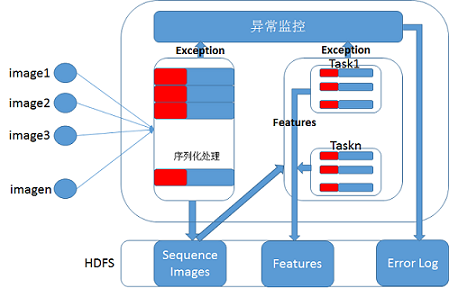
\includegraphics{spark_sift_fw}
\caption{大规模图像库特征提取系统Spark-SIFT系统框架}
\label{fig:spark_sift_fw}
\end{figure}
图像库进行特征提取前,先经过序列化处理模块进行序列化处理,经过序列化模块之后,一张图片转化单条记录的形式,最后将所有的记录序列化保存到分布式文件系统HDFS 中。当进行特征提取时,特征提取功能模块读取HDFS中序列化图片记录,将其分发到各个任务上,任务运行在整个集群上,每个任务上通过Spark-SIFT算法进行特征提取,完成特征提取后,每个task 直接将提取出来的特征保存到HDFS中。Spark-SIFT系统中的异常监控模块收集特征提取作业运行过程中出现的异常信息,将异常信息写到特定的异常日志中。

从软件架构的角度看整个系统,系统的框架图如图\ref{fig:spsift_core_fw}所示,
\begin{figure}[htp]
\centering
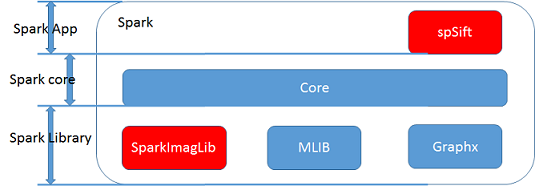
\includegraphics{spsift_core_fw}
\caption{Spark-SIFT软件架构}
\label{fig:spsift_core_fw}
\end{figure}
本文的主要工作在于Spark的库层和应用层。本文实现了Spark下的图像处理基础库Spark-imageLib,这个库包含了spark的图像的表示,读取操作及一些基础的图像处理接口,比如图像的灰度化,图像的缩放,图像的模糊等;这个库和spark的其他库,比如分布式图计算处理库GraphX,机器学习库MLib的地位是等价的,我们已经将该库嵌入到spark的生态系统中。此在这个库的基础上,开发了Spark-SIFT 算法,该算法在Spark 应用中被调用,实现分布式的特征提取工作,图中的spSift就是特征提取应用,它位于Spark的应用层。
\section{系统模块设计}
在本小节中,会详细介绍每个模块的设计及实现,它们分别是spark图像基础库Spark-imageLib,Spark-sift算法,序列化模块,存储模块以及系统容错模块。
\subsection{spark图像基础库spark-imageLib}
Spark-imageLib图像处理库主要包括图像的表示,图像的读取,特征点的表示。
\subsubsection{图像表示}
在图像表示中,本文设计主要用到了三个类,分别是SpImage,SpSingleBandImage及SpFImage,它们间的继承关系如图\ref{fig:image_represent}所示:
\begin{figure}[htp]
\centering
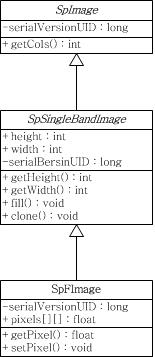
\includegraphics{image_represent}
\caption{Spark下图像表示}
\label{fig:image_represent}
\end{figure}
SpImage为最基础的抽象类,不会直接被使用。SpSingleBandImage为SpImage的子类,它也为抽象类,SpSingleBandImage表示单通道类型的图像。SpFImage 类为SpSingleBandImage 的子类,也是本文中实际用来在Spark下表示图像的类。这三个类都有一个共同的属性变量,就是serialVersionUID,因为本文是一个分布式的图像处理框架,必然会涉及到处理图像文件的网络传输,因此表示图像的类必须是序列化的,这样才能使得图像可以在Spark这个分布式框架下处理。这里的序列化采用的java的序列化方式,因为序列化必然会存在一个反序列化的过程,比如从Master 将图像序列化传送的Worker上,然后Worker 将接受到的内容反序列化得到原始图像,为了避免两端实体类的内容不一样,就使用了serialVersionUID 作为衡量的标准。当JVM获取传来的字节流时,先读取serialVersionUID,然后和本地的进行比较,根据比较的结果判断是否可以进行序列化。

考虑传输过程中的耗费代价,因此设计SpFImage数据结构时要十分精简,在成员变量中,只设置了一个二维数组pixels,这个数组就是保存整张图片的像素信息。因为考虑到高斯模糊时候的精度问题,所以pixels采用了float类型。SpFImage的构造函数是比较灵活的,它允许传递一维数组或者是二维数组,数组的类型是byte或者float,对于不同的参数类型,本文都会自动进行转换。

表\ref{tab:SpFImage_function}列出三个类的主要功能函数:
\begin{table}[h] %开始一个表格environment,表格的位置是h,here。
\caption{SpFImage 主要功能函数} %显示表格的标题
\centering
\label{tab:SpFImage_function}
\begin{tabular}{p{4cm}|p{2cm}|p{6cm}} %设置了每一列的宽度,强制转换。
\hline
\hline
函数名  & 所属类 & 功能 \\ %用&来分隔单元格的内容 \\表示进入下一行
\hline %画一个横线,下面的就都是一样了,这里一共有4行内容
abs  & SpFImage & 对图片的像素点进行绝对值操作\\
\hline
addInplace  & SpFImage & 将图片的像素进行加操作\\
\hline
subtractInplace  & SpFImage & 将图片的像素进行减操作\\
\hline
multiplyInplace  & SpFImage & 将图片的像素进行乘操作\\
\hline
divideInplace  & SpFImage & 将图片的像素进行乘操作\\
\hline
fill  & SpFImage & 对图片进行填充操作\\
\hline
getDoublePixelVector & SpFImage & 将图片像素以一维向量的形式返回\\
\hline
getPixel& SpFImage & 获取图片某个位置上的像素值\\
\hline
setPixel & SpFImage & 对图片某个位置的像素进行赋值\\
\hline
threshold & SpFImage & 对图片像素进行阈值判断\\
\hline
\hline
\end{tabular}
\end{table}
\subsubsection{图像的读取}
在图片读取这个模块中,主要使用到SpImageUtilities 类型,该类提供了从字节流到SpFImage的转换接口,该类的主要成员函数表\ref{tab:SpImageUtilities_function}所示。
\begin{table}[h] %开始一个表格environment,表格的位置是h,here。
\caption{SpImageUtilities 主要功能函数} %显示表格的标题
\centering
\label{tab:SpImageUtilities_function}
\begin{tabular}{p{3cm}|p{3cm}|p{6cm}} %设置了每一列的宽度,强制转换。
\hline
\hline
函数名  & 所属类 & 功能 \\ %用&来分隔单元格的内容 \\表示进入下一行
\hline %画一个横线,下面的就都是一样了,这里一共有4行内容
readF  & SpImageUtilities & 将字节流转化成SpFImage\\
\hline
createFImge  & SpImageUtilities & 将BufferedImage类型的图片转换成SpFImage类型\\
\hline
createBufferImage & SpImageUtilities & 将SpFImage类型图片转换成BufferImage图片\\
\hline
checkSize  & SpImageUtilities & 对图片的大小进行检查\\
\hline
\hline
\end{tabular}
\end{table}

因为图片库是保存在HDFS中的,因此需要用特定的HDFS 接口进行读取,在读取完之后在使用SpImageUtilities 接口进行转换。在HDFS读取接口中,可以通过三个接口进行图片的读取,它们分别是,sequenceFile,binaryFiles及objectFile函数。sequenceFile是spark下用来读取序列化文件的接口,具体定义如下:
\begin{lstlisting}[language=Java,numbers=none]
def sequenceFile[K,V](path:String,KeyClass:Class[K],valueClass:Class[V],minPartitions:Int):RDD[(K,V)]=withScope{}
\end{lstlisting}
sequenceFile保存的是Writable对象,换句话讲,key 和value也必须是Writable类型的,表\ref{tab:Writable}列出了常见类型的Writable对应类型。
\begin{table}[h] %开始一个表格environment,表格的位置是h,here。
\caption{Writable对应类型} %显示表格的标题
\centering
\label{tab:Writable}
\begin{tabular}{p{4cm}|p{2cm}|p{6cm}} %设置了每一列的宽度,强制转换。
\hline
\hline
Scala类型  & Java类型 & Writable类型 \\ %用&来分隔单元格的内容 \\表示进入下一行
\hline %画一个横线,下面的就都是一样了,这里一共有4行内容
Int  & Integer & IntWritable\\
\hline
Long  & Long & LongWritable\\
\hline
Float  & Float & FloatWritable\\
\hline
Double  & Double & DoubleWritable\\
\hline
Array[Byte]  & byte[] & BytesWritable\\
\hline
String  & String & Text\\
\hline
List[T] & List<T> & ArrayWritable\\
\hline
Array[T] & T[] & ArrayWritable\\
\hline
\hline
\end{tabular}
\end{table}

本文设计中,采用sequenceFile读取图片的主要代码如下:
\begin{lstlisting}[language=Java,numbers=none]
val fn_rdd = sc.sequnceFile(imageSEQ_path,classOf[Text],classOf[BytesWritable],task_size.toInt)
.map({case (fname,fcon)} => {
  var datainput:InputStream = new ByteArrayInputStream(fcontext.getBytes)
  var img = SpImageUtilities.readF(datainput)// 读取图片的像素矩阵
...
})
\end{lstlisting}
采用binaryFiles接口进行读取时,返回的是一个key-value类型的RDD,key为文件名,而value则是文件的内容的字节流,binaryFiles的定义如下:
\begin{lstlisting}[language=Java,numbers=none]
def binaryFiles(path:String,minPartitions:Int = defaultMinPartitions):RDD[(String,PortableDataStream)]=withScope{}
\end{lstlisting}
使用binaryFiles接口读取图像的主要代码如下:
\begin{lstlisting}[language=Java,numbers=none]
 sc.binaryFiles(initImgs_path_hdfs,task_size.toInt).map(f => {
      val fname = new Text(f._1.substring(prefix_path_hdfs.length,f._1.length))// 获取features key
      val bytes = f._2.toArray()

      var datainput:InputStream = new ByteArrayInputStream(bytes)
      var img = SpImageUtilities.readF(datainput)
      ...
}
)
\end{lstlisting}
objectFile读取的是对象文件,保存的时候以什么对象类型保存,就以什么类型读取读出,该函数看似是对SequenceFile的简单封装,它运行存储只包含值的RDD,两者的区别在于objectFile保存对象时是采用java序列化的方式,SequenceFile采用的则是hadoop的序列化方式。 objectFile 函数定义如下:
\begin{lstlisting}[language=Java,numbers=none]
def objectFile(path:String,minPartitions:Int = defaultMinPartitions):RDD[T]=withScope{}
\end{lstlisting}
使用objectFile接口读取图像的主要代码如下:
\begin{lstlisting}[language=Java,numbers=none,frame=none]
sc.objectFile(initImgs_500k_path_hdfs).map(x => {
    val test:SpFImage = x
    ...
})
\end{lstlisting}
虽然objectFile读取图像十分方便,但是如果直接将对象保存到HDFS中,储存空间相当大,存储的时间也十分长。
\subsubsection{特征点表示}
%%加上序列化的内容,Hadoop下怎样序列化
在本文设计中,特征点的表示主要涉及到三个模块,分别是SpKeypoint,SpMemoryLocalFeatureList,SpLocalFeatureList。SpKeypoint表示一个sift特征点,SpMemoryLocalFeatureList保存整张图片的sift 特征点,SpLocalFeatureList为接口,SpMemoryLocalFeatureList是SpLocalFeatureList 的具体实现。SpKeypoint成员结构如图\ref{fig:spkeypoint}所示:
\begin{figure}[htp]
\centering
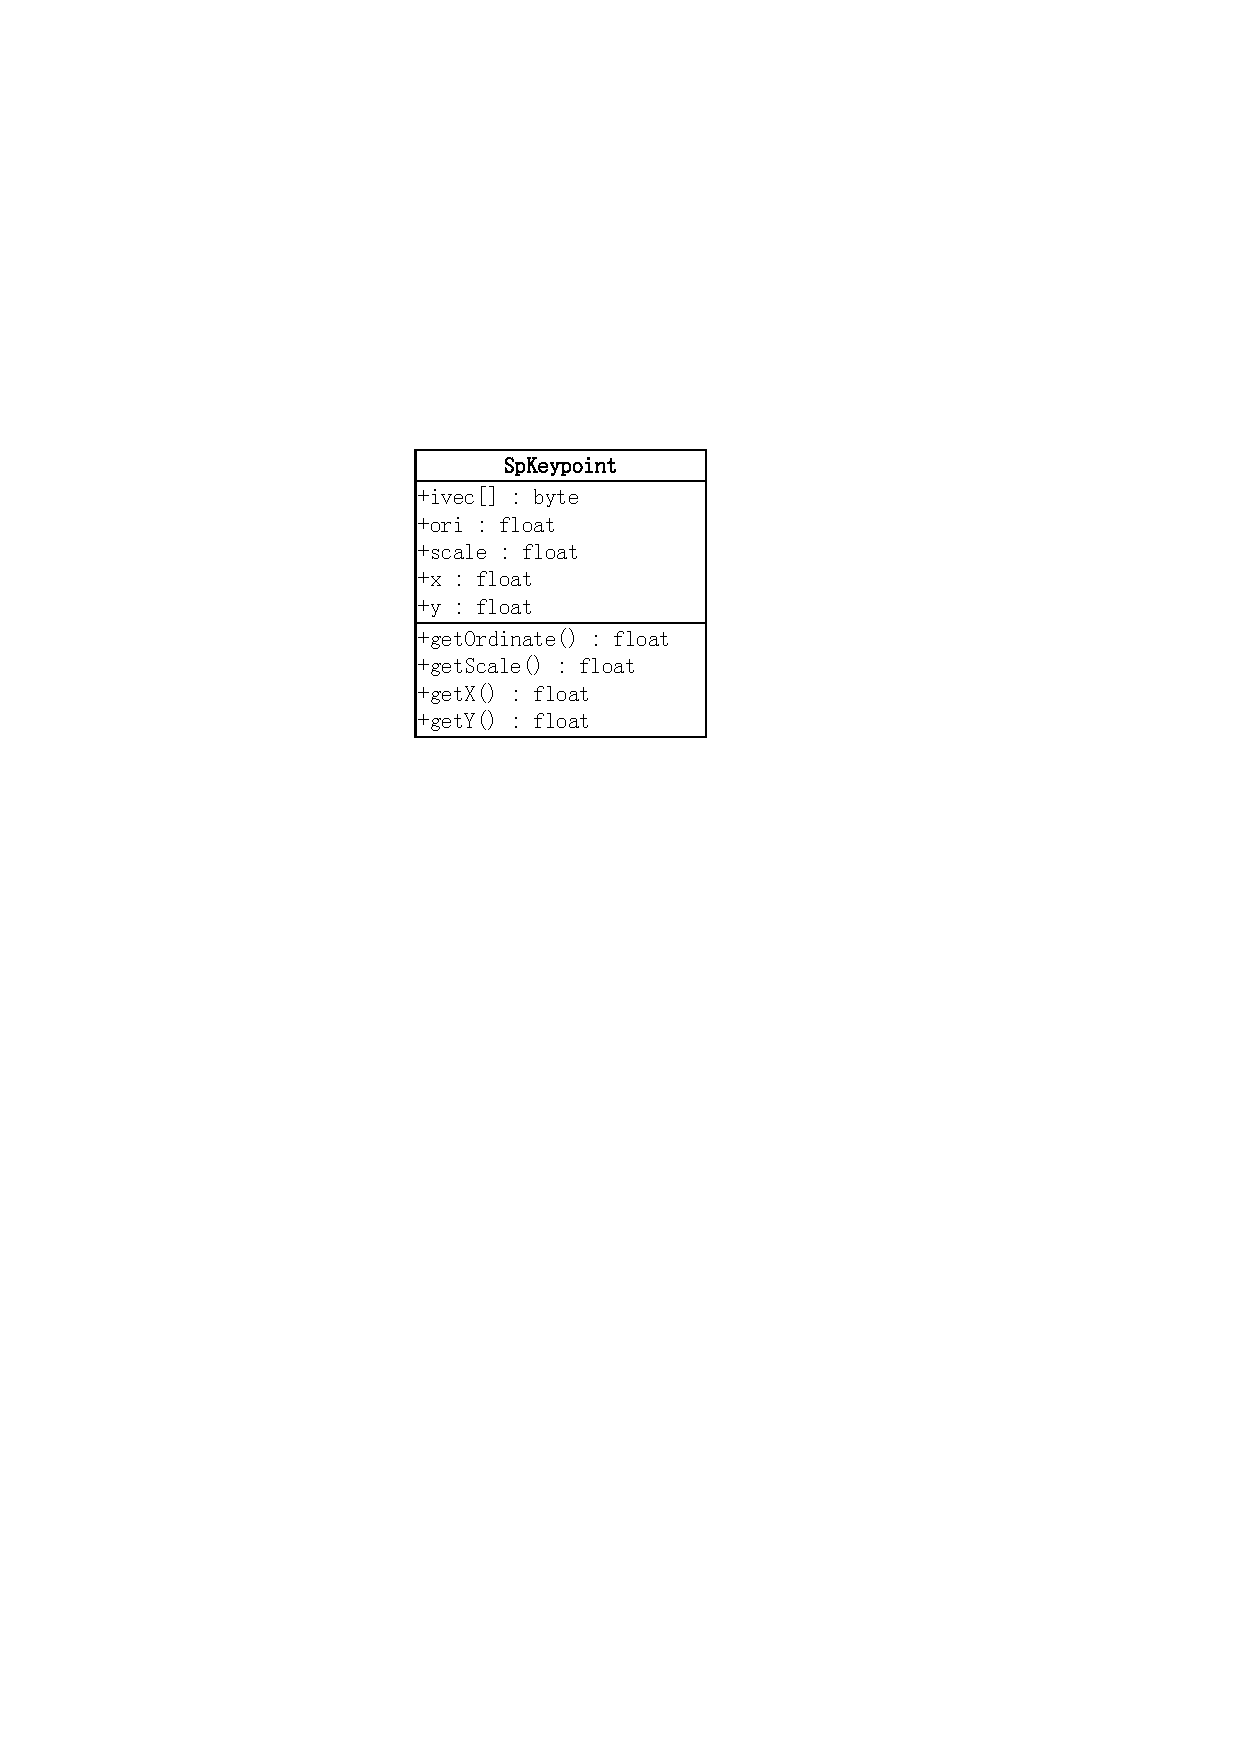
\includegraphics{spkeypoint}
\caption{SpKeypoint数据结构}
\label{fig:spkeypoint}
\end{figure}

其中x,y代表特征点在图片上的坐标,scale表示特征点的尺度大小,ori表示特征点的方向,ivec数组为特征点的一维描述向量,长度为128。

SpMemoryLocalFeatureList数据结构保存SIFT算法检测一张图片得到的所有特征点集,因此SpMemoryLocalFeatureList具有集合特性,本文设计时,让该类继承ArrayList,图\ref{fig:spmemflist} 为SpMemoryLocalFeatureList的UML视图。
\begin{figure}[htp]
\centering
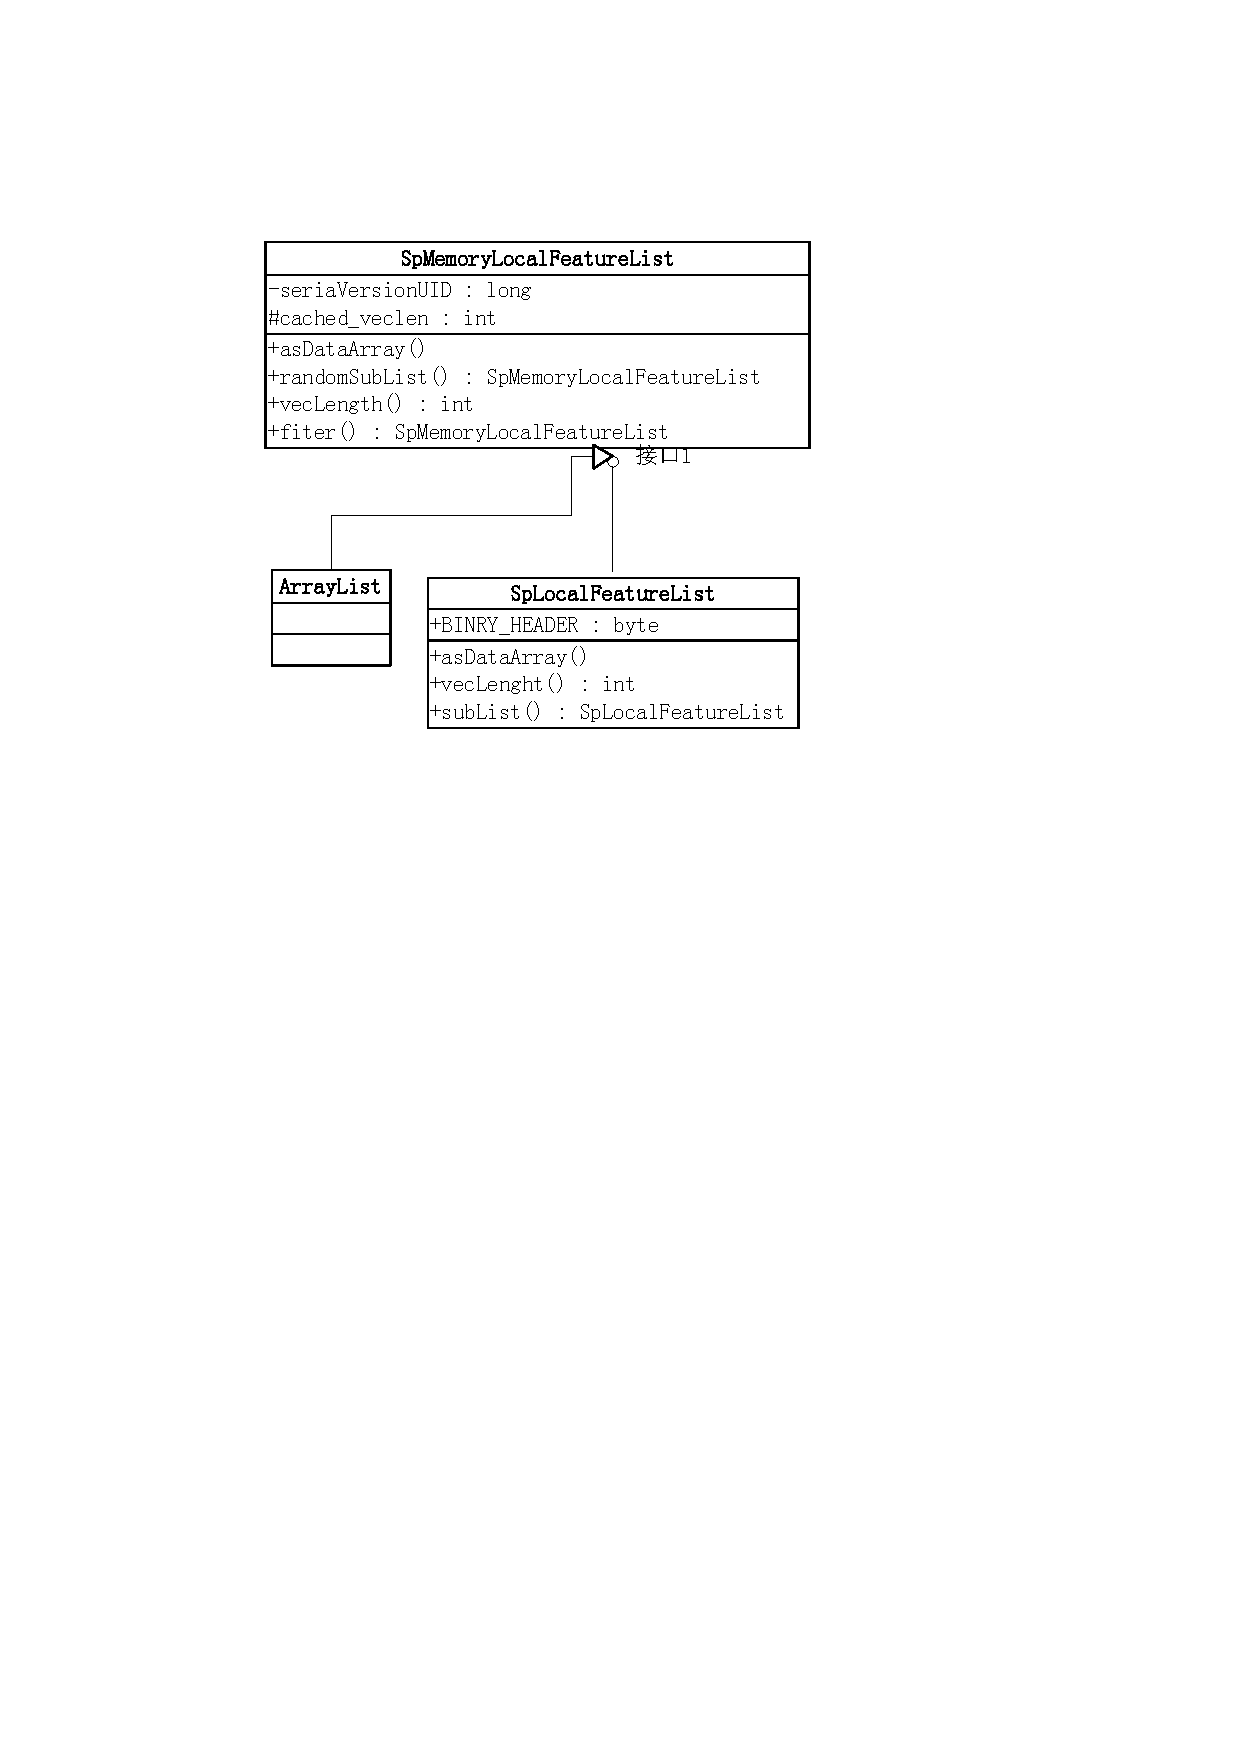
\includegraphics{SpMemoryLocalFeatureList}
\caption{SpMemoryLocalFeatureList数据结构}
\label{fig:spmemflist}
\end{figure}

\subsection{Spark-sift算法}
在这小节中将介绍spark下怎样使用sift算法进行大规模图像库特征提取工作。主要的思想是利用上一小节介绍的spark-imagelib来实现整个SIFT算法,SIFT算法在第二章原理分析中已经详细的分析过了,在此不再详述,然后利用spark的Map-Reduce框架,在map函数中调用已经实现好的SIFT算法,在提取结束后,将特征向量保存到HDFS中,完成整个特征提取的工作。Spark-sift 算法如图\ref{fig:alg_sparksift}所示:
\begin{figure}[htp]
\centering
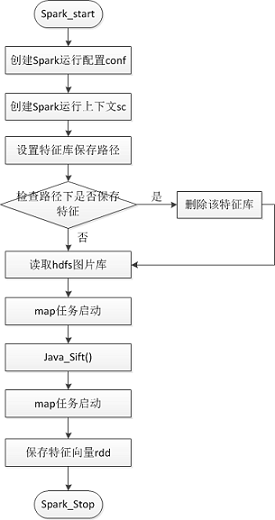
\includegraphics[width=86mm,height=183mm]{alg_sparksift}
\caption{spark-sift算法流程}
\label{fig:alg_sparksift}
\end{figure}

spark-sift算法的关键伪代码如下:
\begin{lstlisting}[language=Java]
val conf = new SparkConf()//创建spark configure
conf.set()//设置configure
val sc = new SparkContext(conf)//创建spark 运行上下文

rm_hdfs(hdfs_name,kpslibdir+dataset)//删除原有的特征库

//并行执行图片特征提取任务
val fn_rdd = sc.sequenceFile(imageSEQ_path,task_size.toInt).map({
var datainput = new ByteArrayInputStream(fcontext.getBytes)

var img = SpImageUtilities.readF(datainput)
if(img != null){
    var engine = new SpDoGSIFTEngine()//进行sift 特征提取
    var kps = engine.findFeatures(img)

    val baos = new ByteArrayOutputStream()
    IOUitls.writeBinary(baos,kps)
    (new Text(fname.toString), new BytesWritable(baos.toByteArray))//以key-value形式返回提取的特征点,key为图片名,value为特征点集
}
})
\end{lstlisting}

通过上面这段代码,每张图片将被划分到不同的分区中,在每个分区中,执行特征提取任务,然后将得到的特征点以Key-Value的形式分布式保存到HDFS中,其中key为图片的文件名,value为特征点集的字节流。
\subsection{序列化模块}
因为互联网上图片的体积一般都是1M以下,HDFS以Block形式进行存储,Block的大小是128M,因此这些文件对于HDFS来说都是小文件,众多的小文件存在时,就会造成频繁的磁盘IO,从而导致读写的性能降低。其实,这种场景在我们生活中也有体会,从U盘拷贝一个2G的文件和拷贝一个由很多小文件组成的2G文件夹,速度是相差很大的。

基于上述情况,本文在整个系统中加入了图片序列化模块,通过该模块将图片转化为Key-Value记录的形式,然后将众多的记录合并并且序列化保存到HDFS中,后续的处理都是在该序列化后的记录上进行,从而提升HDFS 读写效率。本文会在第四章的性能优化中对序列化优化方案进行详细分析,在这里,主要介绍代码框架设计。序列化模块流程框架如图所示\ref{fig:alg_sequence}。
\begin{figure}[htp]
\centering
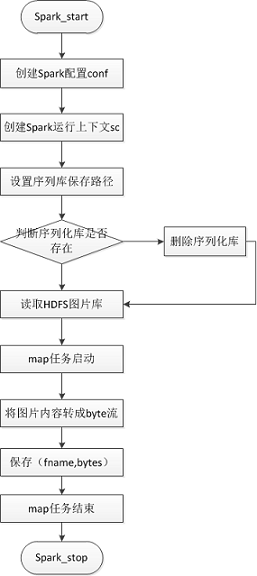
\includegraphics[width=86mm,height=183mm]{alg_sequence}
\caption{序列化模块流程框架图}
\label{fig:alg_sequence}
\end{figure}

序列化模块关键伪代码如下:
\begin{lstlisting}[language=Java]
val conf = new SparkConf()//创建spark configure
conf.set()//设置configure
val sc = new SparkContext(conf)//创建spark 运行上下文

rm_hdfs(hdfs_name,path)//删除原有的序列库

//并行执行图片特征提取任务
val fn_rdd = sc.binaryFiles(initImgs_path,task_size.toInt).map(f =>{
val fname = new Text(f._1.substring(prefix_path_hdfs))//构造记录的key值

val bytes = f._2.toArray()
val fcontext = new BytesWritable(bytes)//将图片的内容转化成byte字节流

(fname,fcontext)//以序列化方式保存图片到hdfs
}).saveAsHadoopFile(path)
\end{lstlisting}

通过上面这段序列化预处理代码,每张图片将划分到不同的分区,在不同的分区中执行图片转成单条记录的形式的任务,最后记录以Key-Value的形式保存到HDFS 中。
\subsection{存储模块}
在存储层设计,本文采用HDFS当作系统的存储层,将图像库,图像序列化库,图像特征集,错误信息均保存到HDFS中。因为面对着大规模数据时,单机存储的方案基本是不太现实的,所以本文采用了分布式的存储方案。HDFS是Hadoop下的产物,但是它和Spark的交互也十分方便。spark下提供有丰富的HDFS 操作API,通过这些API,基本上能满足开发者的需求。本文设计主要用到了HDFS的以下接口:
\begin{table}[h] %开始一个表格environment,表格的位置是h,here。
\caption{Spark-SIFT系统涉及的HDFS API} %显示表格的标题
\centering
\label{tab:HDFS_API}
\begin{tabular}{p{3cm}|p{8cm}} %设置了每一列的宽度,强制转换。
\hline
\hline
函数名  &  功能 \\ %用&来分隔单元格的内容 \\表示进入下一行
\hline %画一个横线,下面的就都是一样了,这里一共有4行内容
sequenceFile   & 读取hdfs序列化后的图片\\
\hline
binaryFiles   & 读取hdfs图片库图片\\
\hline
saveAsHadoopFile  & 将图片或者是特征点集以序列化方式保存到hdfs\\
\hline
FileSystem.get & 获取hdfs文件的句柄\\
\hline
FileSystem.delete & 删除hdfs文件\\
\hline
\hline
\end{tabular}
\end{table}
\subsection{容错模块}
在大数据处理中,系统的容错是一个十分重要的功能,因为处理的数据量太大,处理的时间太长,因此处理过程中发生一些错误是十分常见的情况,比如有可能处理的数据中有几个非法的数据,在Spark-SIFT系统处理过程中,我们经常就会碰到图片集合中有几张非法格式的图片。但是系统不能因为这个非法格式的数据而处理被中断或者是崩溃,因此大数据系统中应该有一套自己的容错机制。在Spark-SIFT中,系统中有一个模块会对图片格式的合法性进行判断,找出所有非法格式的图片,然后将这些文件名连同路径写到HDFS中非法文件保存目录下,系统会定期读取该目录,进行非法格式图片的删除。

在Spark中如果应用运行的过程出现了运行时的异常,应用会直接退出。因此针对这种情况,在Spark-SIFT系统进行特征提取时,我们对特征提取应用的每一个stage都加入了过滤功能,将一些非法的结果过滤掉,只传送合法的结果到下一个stage,这样系统就不会因为发生异常而直接退出。具体实现时,本文是采用了Scala中的Try异常捕捉机制,当采用这种异常捕捉机制时,结果的返回一个重新封装的数据结构,该数据结构包含正确和异常的两个结果,换而言之,什么类型的结果都会返回,具体需要什么,我们可以根据条件进行过滤删选。图\ref{fig:try_stage}显示了Spark-SIFT系统在一个stage结束之后调用容错处理操作。
\begin{figure}[htp]
\centering
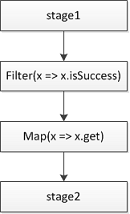
\includegraphics{try_stage}
\caption{stage和stage间的容错处理}
\label{fig:try_stage}
\end{figure}
%%需要做一些工作
\section{系统执行与验证}
在这小节中将会介绍整个Spark-SIFT大规模特征提取系统的编译,执行及正确性验证。
\subsection{spark-imageLib编译}
本文设计的图像基础库需要嵌入到spark系统中,因此需要和Spark的源码一块编译,然后在Spark应用开发中,以依赖的形式导入Spark-imageLib库支持。本文使用的Spark版本是2.0.0,其源代码可以在Spark 官网或者是github网站下载。Spark源码是一个maven工程,maven是一个高级的项目管理工具,可以管理项目中的所有依赖及其他配置。下面简要的介绍一下创建Spark-imageLib的步骤:
\begin{compactenum}
\item 在Spark源码根目录下创建一个新的maven工程,工程的groupId为org.apache.spark,artifactId为spark-imageLib\textunderscore2.11;
\item 修改spark源码根目录下的pom.xml文件,在modules配置项中加入module值为imageLib的配置项;
\item 编译源代码,编译命令为mvn clean install,该命令会重新编译Spark源码,生成新的spark安装包,我们需要将新的spark安装包安装在集群上;
\end{compactenum}
\subsection{特征提取应用程序提交}
在Spark特征提取应用程序中引用Spark-imageLib库依赖,编写特征提取程序,编译生成分布式特征提取应用jar包,然后该jar包提交到Spark运行集群上。提交命令如下:
\begin{code}
spark-submit
\\--class cn.zxm.scala.sparkImageDeal.ImagesFeatureEx
\\--master spark://hadoop0:7077
spark-SIFT-1.0.SNAPSHOT.jar
\end{code}
\subsection{正确性验证}
\begin{figure}[htp]
\centering
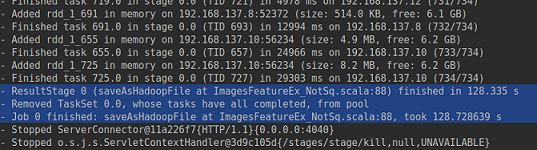
\includegraphics{find_finish}
\caption{提取作业结果}
\label{fig:find_finish}
\end{figure}

\begin{figure}[htp]
\centering
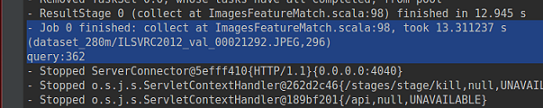
\includegraphics{00021292_match}
\caption{00021292图片匹配结果}
\label{fig:00021292_match}
\end{figure}

以280M的图片数据集为例子,该数据集共有1833张图片,简单展示一下从Spark-SIFT系统的特征提取功能,运行提取作业结果如图\ref{fig:find_finish} 所示。我们从该数据集中随机抽取了4张图片,分别是ILSVRC2012\textunderscore val\textunderscore00021292.JPEG,ILSVRC2012\textunderscore val\textunderscore00021324.JPEG,ILSVRC2012\textunderscore val\textunderscore00021353.JPEG 及ILSVRC2012\textunderscore\\val\textunderscore00021358.JPEG,使用这四张图片去查询匹配以验证提取的特征点的正确性,匹配程序中的匹配条件为匹配特征点数必须大于查询图片特征点的1/2,并且不能超过查询特征点总数。四张图片的匹配结果分别如图\ref{fig:00021292_match},图\ref{fig:00021324_match},图\ref{fig:00021324_match},图\ref{fig:00021358_match}所示,其中第一张图片查询特征点总数为362,匹配查询结果为一张,错误率为0\%,匹配点数为296;第二张图片查询特征点总数为1030,匹配查询结果为一张,错误率为0\%,匹配点数为898;第三张图片查询特征点总数为400,匹配查询结果为一张,错误率为0\%,匹配点数为317;第四张查询特征点数为351,匹配查询结果为5张,错误率为0.27\%,和原图匹配的特征点数为318,在所有的匹配图片中是最高的。

\begin{figure}[htp]
\centering
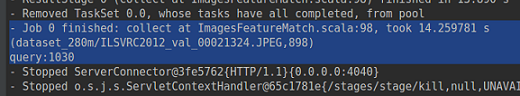
\includegraphics{00021324_match}
\caption{00021324图片匹配结果}
\label{fig:00021324_match}
\end{figure}

\begin{figure}[htp]
\centering
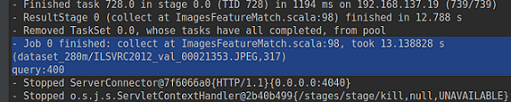
\includegraphics{00021353_match}
\caption{00021353图片匹配结果}
\label{fig:00021353_match}
\end{figure}

\begin{figure}[htp]
\centering
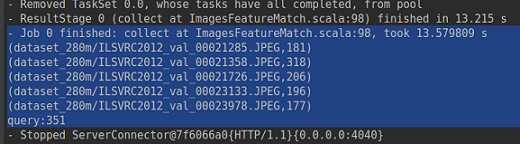
\includegraphics{00021358_match}
\caption{00021358图片匹配结果}
\label{fig:00021358_match}
\end{figure}

\section{本章小结}
本章主要介绍了大规模图像库特征提取系统Spark-SIFT 的设计和实现,首先介绍了系统的主要框架,从软件架构的角度分析了系统的每一个模块的设计和实现,分别介绍了Spark-imageLib,Spark-sift算法,序列化模块,存储模块以及容错模块。最后展示了特征提取系统的编译执行及提取结果。
